\chapter{An Atlas of the Theorems: Graph and Retrieval Analysis}\label{ch:atlas}

The formalization described in \cref{ch:architecture} is not one library but seven, written
over many months by different people and by the tiered pipeline of \cref{ch:pipeline}.
Together they compile to $1224$ declarations, of which $423$ are theorems written by hand
in the source \source{atlas.md, l.~3}. A student who opens this code base faces the same
problem as one who opens a large physics literature: which results are load-bearing,
which are restatements, which two results that \emph{look} the same are in fact one, and
which two results that look different secretly rest on the same lemma. This chapter
answers those questions with two tools borrowed from data analysis, a dependency graph
and a text-retrieval index, and, more importantly, shows how to \emph{read} what the
tools return. Every number below is taken from the generated file
\texttt{atlas\_data.json}; where a number is re-derived by hand or by a script we say so.
The chapter is also an inventory of technical debt: the same fact, for instance
$\chi(K3)=24$, is proved independently in six places, and we discuss what that means and
how to repair it.

\section{Two relations between theorems, kept apart}\label{sec:atlas:method}
\index{theorem atlas}\index{dependency graph}

\subsection{The kernel-level dependency graph}

The first relation is \emph{dependency}. A Lean theorem is a term whose type is the
statement; term and type both mention other constants (definitions, lemmas, inductive
types). The extractor \texttt{tools/lean\_depgraph.lean} imports the seven libraries,
walks every constant of the elaborated environment, and for each constant of the project
prints the constants used by its statement (\lean{info.type.getUsedConstants}) and by its
proof or body (\lean{t.value.getUsedConstants}) \source{lean\_depgraph.lean,
ll.~30--55}. Constructors and recursors are skipped; for theorems the extractor also
records the subset of proof dependencies that are theorems of Mathlib or core, called
\texttt{lemmas}, so that the shared foundations of \cref{sec:atlas:shared} are not
drowned in notation constants such as \lean{Neg.neg} \source{lean\_depgraph.lean,
ll.~48--54}. The Python side then discards auto-generated names
(\lean{.rec}, \lean{.casesOn}, \lean{.sizeOf\_spec}, \dots) and keeps as ``theorems''
only those kernel theorems that are also written as \lean{theorem} in a source file,
so that structure projections and equation lemmas are not counted
\source{theorem\_atlas.py, ll.~38--40, 76--79}.

\begin{pitfallbox}[Regex is not dependency]
An earlier tool inferred edges by searching source text for names. That misses edges
created by \lean{simp} sets and by tactics such as \lean{omega} and \lean{norm\_num},
which insert Mathlib lemmas never written in the source, and it invents edges from names
in comments. The kernel-level graph has neither defect: an edge exists exactly when the
elaborated term mentions the constant \source{lean\_depgraph.lean, ll.~6--8}. The price
is that it \emph{does} see the scaffolding of every tactic, which is why the weighting
below is needed.
\end{pitfallbox}

Writing $D(a)$ for the set of constants used by the statement or proof of theorem $a$,
the raw Jaccard index $|D(a)\cap D(b)|/|D(a)\cup D(b)|$ would be useless: almost every
theorem uses \lean{Eq}, \lean{OfNat.ofNat} and the arithmetic instances of $\N$ and $\Z$.
The script therefore weights each constant $c$ by its inverse document frequency over the
$N=423$ theorems,
\begin{equation}\label{eq:atlas:idf}
  \operatorname{idf}(c)=\ln\frac{N}{\operatorname{df}(c)},\qquad
  \operatorname{df}(c)=\#\{a:\ c\in D(a)\},
\end{equation}
and defines the \emph{weighted Jaccard index}\index{Jaccard index, weighted}
\begin{equation}\label{eq:atlas:wjacc}
  J(a,b)=\frac{\sum_{c\in D(a)\cap D(b)}\operatorname{idf}(c)}
              {\sum_{c\in D(a)\cup D(b)}\operatorname{idf}(c)}
\end{equation}
\source{theorem\_atlas.py, ll.~106--115}. A constant used by every theorem has
$\operatorname{idf}=0$ and counts for nothing; \lean{Eq} has
$\operatorname{df}=358$ and weight $\ln(423/358)=0.167$, while
\lean{Matrix.fromBlocks\_multiply} has $\operatorname{df}=13$ and weight $3.48$. Sharing
the block-multiplication lemma is twenty times more significant than sharing equality.
Since $0\le J\le1$, with $J=1$ exactly when the two sets agree up to constants of zero
weight (\cref{ex:atlas:jbound}), $J$ is a genuine similarity measure on the graph.

\subsection{The retrieval index}

The second relation is \emph{textual similarity} of statements, the relation a search
engine computes. For each theorem the script forms a bag of tokens from its name (with
underscores and dots replaced by spaces, counted twice), its signature as stored in the
declaration index, and the first $400$ characters of its docstring
\source{theorem\_atlas.py, ll.~151--157}. With $f_t$ the count of token $t$ in a theorem
and $\operatorname{tdf}(t)$ the number of theorems containing $t$, the weight is the
standard TF--IDF\index{TF-IDF}
\begin{equation}\label{eq:atlas:tfidf}
  w_t=\bigl(1+\ln f_t\bigr)\,\ln\frac{N}{\operatorname{tdf}(t)},
  \qquad\text{tokens with }\operatorname{tdf}(t)\ge N/2\text{ dropped},
\end{equation}
and the similarity of two theorems is the cosine of the angle between their weight
vectors, $\cos(a,b)=\sum_t \hat w^{(a)}_t\hat w^{(b)}_t$ with $\hat w=w/\|w\|$
\source{theorem\_atlas.py, ll.~158--169}.

Both relations are computed for all pairs and reported in separate tables
(\cref{sec:atlas:tables}): pairs from different libraries with $\cos\ge0.30$, pairs from
different modules with $J\ge0.35$, and, singled out, pairs with $\cos\ge0.30$ but
$J<0.05$, the \emph{unification candidates}\index{unification candidate}: statements
that read alike whose proofs share essentially nothing
\source{theorem\_atlas.py, ll.~171--185}. Keeping the two relations apart is the main
methodological point of the chapter; the worked examples show why.

\begin{physicsbox}[What the two numbers measure]
Think of a theorem as an experiment. $J$ asks whether two experiments share apparatus:
the same lemmas, definitions and tactic machinery. $\cos$ asks whether their write-ups
use the same words. Two measurements of one quantity with independent apparatus (high
$\cos$, low $J$) are valuable cross-checks but expensive to maintain; two runs on the
same apparatus with different labels (high $J$, low $\cos$) may have nothing in common
physically, they merely used the same voltmeter. Only a pair high on both is a duplicate.
\end{physicsbox}

\section{Worked examples with the actual numbers}\label{sec:atlas:examples}

\begin{example}[Weighted Jaccard of two proofs of $\chi(K3)=24$]\label{ex:atlas:jacc}
Take $a=$ \lean{k3\_euler\_characteristic} of \texttt{DoubleFieldTheory.K3Topology},
which states \lean{K3BettiSum 1 0 22 0 1 = 24} and is closed by \lean{decide}, and
$b=$ \lean{k3\_euler\_eq\_24} of \texttt{SocrateAI.Moonshine}, which states
\lean{k3\_euler = 24} and is closed by \lean{rfl}. Re-running the extraction on the
compiled environment gives $|D(a)|=12$, $|D(b)|=6$ and these weights, with $N=423$:
\begin{center}\small
\begin{tabular}{@{}llrr@{}}\toprule
Constant & in & $\operatorname{df}$ & $\operatorname{idf}$ \\ \midrule
\lean{K3BettiSum} (of $a$'s module) & $a$ & 1 & 6.047 \\
\lean{k3\_euler} (of $b$'s module) & $b$ & 1 & 6.047 \\
\lean{Int.instDecidableEq} & $a$ & 57 & 2.004 \\
\lean{Decidable.decide} & $a$ & 72 & 1.771 \\
\lean{of\_decide\_eq\_true} & $a$ & 73 & 1.757 \\
\lean{Bool.true} & $a$ & 80 & 1.665 \\
\lean{Bool} & $a$ & 93 & 1.515 \\
\lean{instOfNat} & both & 142 & 1.092 \\
\lean{Int} & both & 220 & 0.654 \\
\lean{id} & $a$ & 237 & 0.579 \\
\lean{Eq.refl} & both & 263 & 0.475 \\
\lean{OfNat.ofNat} & both & 349 & 0.192 \\
\lean{Eq} & both & 358 & 0.167 \\
\bottomrule\end{tabular}
\end{center}
The intersection carries weight $1.092+0.654+0.475+0.192+0.167=2.580$; the union carries
$2.580+6.047+(6.047+2.004+1.771+1.757+1.665+1.515+0.579)=23.965$; hence
$J=2.580/23.965=0.108$, the value printed in \cref{tab:atlas-similar}
\source{atlas.md, l.~131}. Read the table: the two theorems share only the vocabulary of
integer equality. Everything specific to $a$ is the \lean{decide} machinery and its own
definition \lean{K3BettiSum}; everything specific to $b$ is its own definition
\lean{k3\_euler}. Neither proof knows the other exists.
\end{example}

\begin{example}[Cosine of the same pair]\label{ex:atlas:cos}
The retrieval side sees the same pair very differently. After tokenizing, the two
theorems share six tokens; the table lists counts, token document frequency, the weight
in $a$, and each token's contribution $\hat w^{(a)}_t\hat w^{(b)}_t$ to the cosine.
\begin{center}\small
\begin{tabular}{@{}lrrrrr@{}}\toprule
Token & $\operatorname{tdf}$ & $f^{(a)}$ & $f^{(b)}$ & $w^{(a)}$ & contribution \\ \midrule
\texttt{euler} & 32 & 4 & 6 & 6.161 & 0.276 \\
\texttt{characteristic} & 22 & 4 & 2 & 7.055 & 0.219 \\
\texttt{int} & 75 & 2 & 2 & 2.929 & 0.053 \\
\texttt{topological} & 27 & 1 & 1 & 2.752 & 0.047 \\
\texttt{theorem} & 32 & 1 & 1 & 2.582 & 0.041 \\
\texttt{def} & 175 & 1 & 1 & 0.883 & 0.005 \\
\bottomrule\end{tabular}
\end{center}
Check one entry: $w^{(a)}_{\texttt{euler}}=(1+\ln4)\ln(423/32)=2.386\times2.581=6.16$.
With $\|w^{(a)}\|=13.93$ and $\|w^{(b)}\|=11.56$ the contributions sum to $0.642$, the
top entry of \cref{tab:atlas-similar} \source{atlas.md, l.~131}. Two tokens,
\texttt{euler} and \texttt{characteristic}, account for $77\%$ of the similarity. The
index has matched the \emph{words}, as it should; whether the mathematics is the same is
a question for the reader, and here the answer is yes: both are the alternating sum
$1-0+22-0+1$. The token \texttt{the} was dropped as occurring in more than half of all
theorems; \texttt{k3} and \texttt{24} are shorter than three characters and are never
tokenized, a limitation worth knowing when a search for ``24'' returns nothing.
\end{example}

\begin{example}[High dependency overlap, no textual similarity]\label{ex:atlas:m24}
The strongest dependency intersection between different modules is $J=0.925$, with
cosine only $0.092$, for \lean{M24\_order} of \texttt{StringTheory.StringDynamics}, which
states \lean{(244823040 : ℕ) = 2\^{}10 * 3\^{}3 * 5 * 7 * 11 * 23}, and
\lean{M21\_order\_factorization} of \texttt{StringTheory.UseCases.MathieuTower}, which
states \lean{orderM21 = 2 \^{} 6 * 3 \^{} 2 * 5 * 7} \source{atlas.md, l.~193}. The
re-run shows $D(a)\subset D(b)$: all $26$ constants of $a$ are among the $28$ of $b$, the
two extra ones being \lean{orderM21} and \lean{id}. The $26$ shared constants are the
internals of \lean{norm\_num} (\lean{isNat\_mul}, \lean{isNat\_pow},
\lean{IsNatPowT.bit0}, \dots) and the semiring instances of $\N$. Both facts are true
(\cref{ch:m24}), but the graph says only that both were proved by the same tactic. This
is the case the weighting cannot remove: \lean{norm\_num} internals are rare enough
across the corpus to carry weight, so two factorization checks look like close relatives.
A high $J$ with a low cosine means ``same apparatus'' and nothing more.
\end{example}

\begin{example}[A genuine duplicate]\label{ex:atlas:dup}
\lean{buscher\_log\_involution} of \texttt{DoubleFieldTheory.TDualityBuscher} states
\lean{BuscherLogMap (BuscherLogMap x) = x} for \lean{x : Int}, where \lean{BuscherLogMap}
is negation; \lean{buscher\_log\_involution} of \texttt{DualScaleValidation.UseCase1}
states \lean{-(-x) = x}; both are closed by \lean{omega}. The pair scores $\cos=0.445$
\emph{and} $J=0.351$ \source{atlas.md, l.~145}: same words, same apparatus, a true
duplicate. Physically both encode $\ln R\mapsto-\ln R$, the statement that
$R\mapsto\ap/R$ is an involution (\cref{ch:tduality}), reduced to the arithmetic shadow
$-(-x)=x$ on integers.
\end{example}

\section{The module graph and the hubs}\label{sec:atlas:hubs}
\index{hub declaration}\index{module graph}

Aggregating the constant-level edges by module gives \cref{fig:atlas:modules}: $44$
modules joined by $42$ directed edges, an edge $M\to M'$ meaning that some declaration of
$M$ mentions a declaration of $M'$, drawn thicker when more do
\source{theorem\_atlas.py, ll.~188--201}. Modules without edges are omitted. Three
features stand out. First, the graph is a forest of shallow trees; the deepest chain is
\texttt{TDuality.Spectrum} $\to$ \texttt{DFT.GeneralizedMetric} $\to$ \texttt{TDuality.ODD}
$\to$ \texttt{Lattice.Hyperbolic} $\to$ \texttt{Lattice.Basic}, continuing across the
library border into Stream 1's \texttt{UseCases.NarainLattice} and
\texttt{UseCases.TDualityMassSpectrum} \source{module\_graph.dot}. Second,
\texttt{DualScaleStream2} is the only library organized as a tree, with two roots:
\texttt{Lattice.Basic} (the Gram-matrix predicates of \cref{ch:lattices}) and
\texttt{TDuality.ODD} (the group $\Odd{d}$ of \cref{ch:odd}). Third, four of the seven
libraries, \texttt{DoubleFieldTheory}, \texttt{DualScaleM24Formalization},
\texttt{DualScaleValidation} and \texttt{Lean5Corpus}, have no edge to any other library:
they are islands, the structural reason for the duplication of \cref{sec:atlas:unify}.

\begin{figure}[p]
\centering
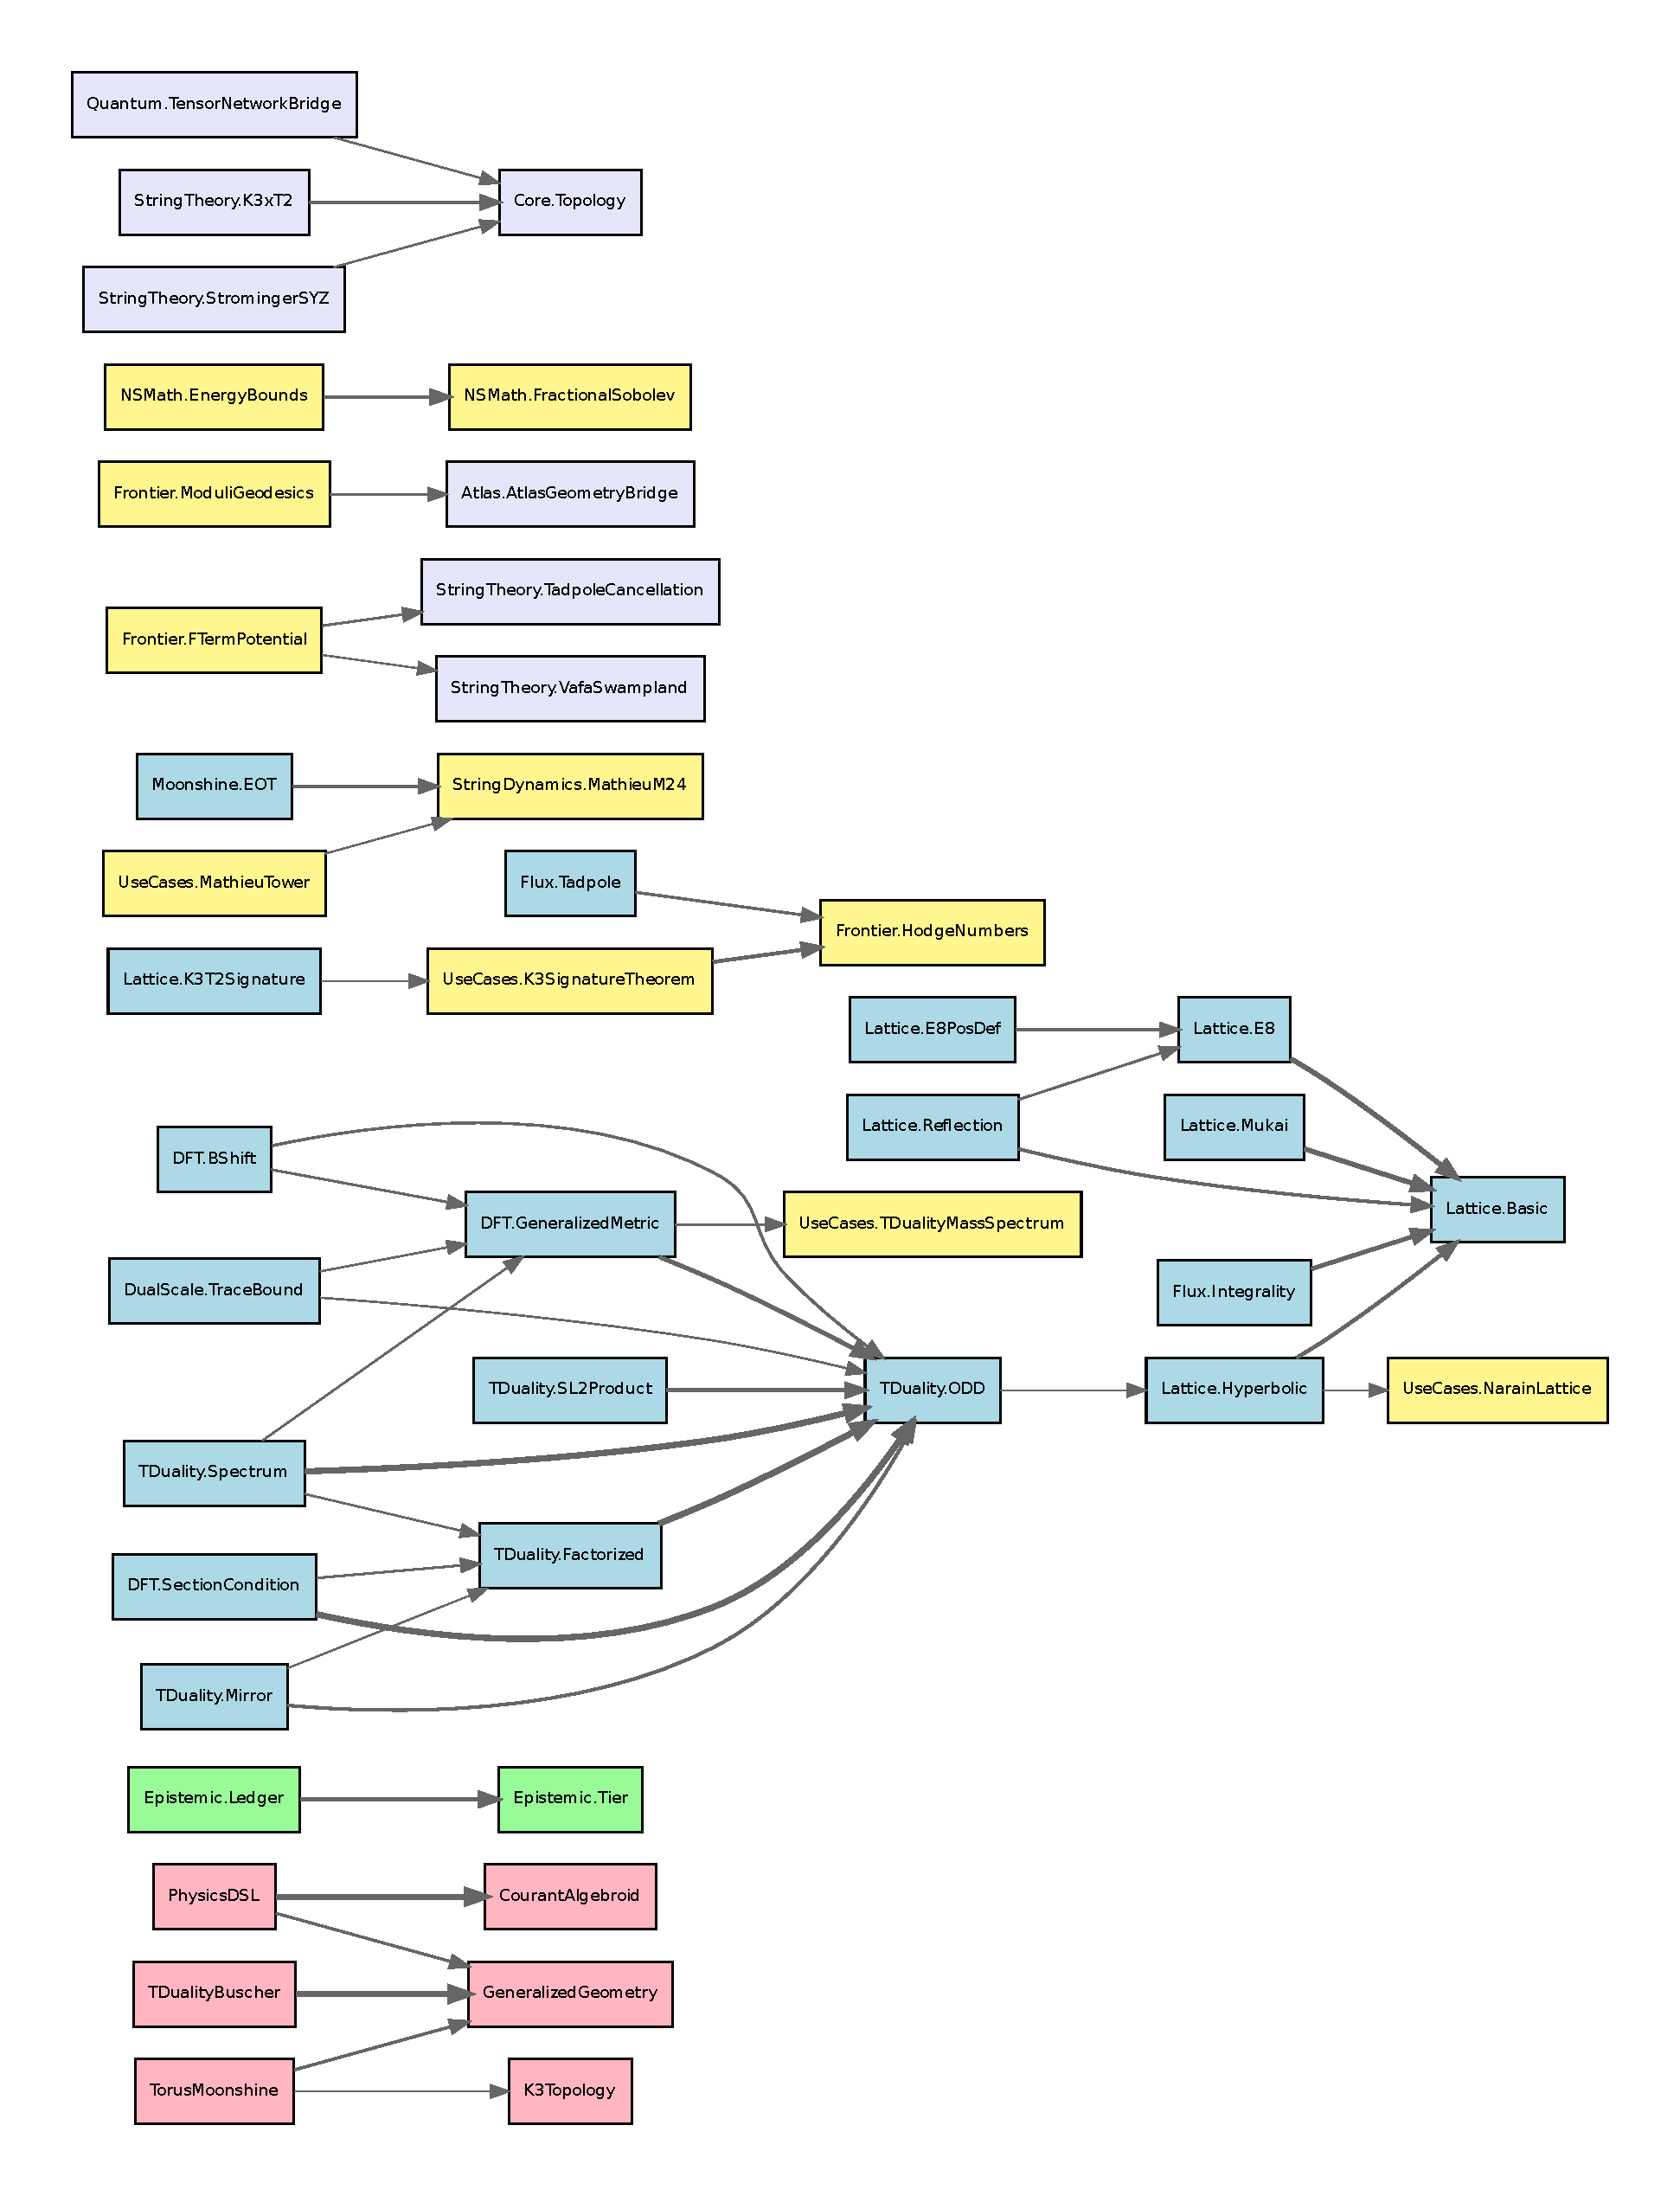
\includegraphics[width=\textwidth]{generated/module_graph.pdf}
\caption{Module-level dependency graph extracted from the kernel: $44$ modules, $42$
edges. Colours mark libraries (blue: \texttt{DualScaleStream2}; yellow:
\texttt{StringTheoryFormalization}; pink: \texttt{DoubleFieldTheory}; green:
\texttt{DualScaleM24Formalization}; lavender: \texttt{StringTheoryFoundation}). An arrow
from $M$ to $M'$ means a declaration of $M$ uses a declaration of $M'$. Generated by
\texttt{tools/theorem\_atlas.py} from \texttt{.leancache/depgraph.jsonl}; the source PDF
is legible at higher magnification.}
\label{fig:atlas:modules}
\end{figure}

A \emph{hub} is a declaration of the project used by many of the project's theorems.
\Cref{tab:atlas-hubs} lists the forty largest; the top is \source{atlas.md, ll.~6--11}:
\begin{center}\small
\begin{tabular}{@{}llrp{6.4cm}@{}}\toprule
Declaration & Kind & Used by & What it is \\ \midrule
\lean{TDuality.Charge} & def & 36 & the index type $\mathrm{Fin}\,d\oplus\mathrm{Fin}\,d$ of $(n,w)$ \\
\lean{TDuality.eta} & def & 20 & $\eta=\bigl(\begin{smallmatrix}0&\mathbf 1\\ \mathbf 1&0\end{smallmatrix}\bigr)$ over $\Z$ \\
\lean{Lattice.Gram} & def & 20 & integer $n\times n$ Gram matrices \\
\lean{Frontier.k3HodgeNumber} & def & 12 & the $3\times3$ Hodge table of K3 \\
\lean{TDuality.IsODD} & def & 12 & the predicate $g^{\mathsf T}\eta g=\eta$ \\
\lean{Epistemic.Tier} & inductive & 11 & the five-valued tier type of the ledger \\
\bottomrule\end{tabular}
\end{center}
Each hub is a \emph{definition}, not a theorem, and each is a piece of the mathematics of
\cref{ch:odd,ch:lattices,ch:k3}. The largest, \lean{Charge}, is only a type,
\lean{abbrev Charge (d : ℕ) := Fin d ⊕ Fin d} \source{TDuality/ODD.lean, l.~75}. That a
type with no content is the most-used object is not a paradox: every statement about a
$2d\times2d$ block matrix, over $\Z$ in \texttt{TDuality} or over $\R$ in \texttt{DFT},
is indexed by it, so the count $36$ measures the size of the block-matrix formalization,
not the importance of a theorem. The definitions \lean{eta}, \lean{IsODD}, \lean{Gram}
are the working hubs from which the duality group and the lattice theory hang.
\lean{k3HodgeNumber} is a hub of a different kind: a hand-written table
\lean{Fin 3 → Fin 3 → ℕ} with entries $h^{0,0}=h^{2,0}=h^{0,2}=h^{2,2}=1$, $h^{1,1}=20$,
the rest $0$, which its file describes as ``asserted, not derived''
\source{Frontier/HodgeNumbers.lean, ll.~99--112}. Twelve theorems in two libraries rest on
it, including the tadpole arithmetic of \cref{ch:tadpole}; a mistyped entry would make
all twelve wrong together. A hub concentrates risk as well as reuse.

The hub \lean{SocrateAI.Epistemic.Tier} deserves a warning. It is the ledger's own tier
type with five constructors \lean{X}, \lean{C}, \lean{L}, \lean{B}, \lean{A}
\source{Epistemic/Tier.lean, ll.~16--22}, finer than this book's three badges; the
theorems built on it, such as \lean{no\_kernel\_claim\_rests\_on\_weaker}, are statements
about a finite ordered type and a bookkeeping structure, not about any theorem of the
project. A Lean proof that ``no A-claim depends on a weaker claim'' \emph{inside the
ledger model} is not an audit of the libraries; the audit is the axiom check of
\cref{ch:leanprimer}.

\section{The nineteen bridges}\label{sec:atlas:bridges}
\index{cross-library bridge}

A \emph{bridge} is a theorem whose statement or proof uses a declaration of a different
library. There are $19$, listed in \cref{tab:atlas-bridges}, and they run in only two
directions: $13$ from \texttt{DualScaleStream2} into \texttt{StringTheoryFormalization}
and $6$ from \texttt{StringTheoryFormalization} into \texttt{StringTheoryFoundation}
\source{atlas.md, ll.~48--66}. Grouped by theorem:
\begin{enumerate}[leftmargin=*,itemsep=2pt]
\item \lean{massForm\_circle} (\texttt{DFT}) $\to$ \lean{leftMomentum},
  \lean{rightMomentum}, \lean{momentumMassSq} of Stream 1 (three edges). For rational
  $n,w,R$ with $R\ne0$,
  \[
    \mathrm{massForm}\bigl(\HH(R^2,0),(w,n)\bigr)=\tfrac12\,\mathrm{momentumMassSq}(n,w,R),
  \]
  the DFT mass form of \cref{ch:genmetric} on a circle equals half of Stream 1's
  $p_L^2+p_R^2$ of \cref{ch:circle} \source{DFT/GeneralizedMetric.lean, ll.~184--189}.
  Two formalizations of the circle spectrum, written independently with different
  conventions (the DFT charge vector is $(w,n)$), are proved to agree; the factor
  $\tfrac12$ is the usual one between $Z^{\mathsf T}\HH Z$ and $p_L^2+p_R^2$.
\item \lean{euler\_K3}, \lean{k3k3\_anomaly}, \lean{k3t2\_euler\_zero}
  (\texttt{Flux}) $\to$ \lean{k3HodgeNumber}. Stream 2 does not retype the Hodge diamond;
  it applies its own functional \lean{eulerFromHodge} to Stream 1's table and gets $24$,
  then $24^2/24=24$ and $24\cdot0=0$ \source{Flux/Tadpole.lean, ll.~86--112}. Bridges by
  \emph{reuse}: one object, two consumers.
\item \lean{hyperbolicU\_eq\_narain\_gram} $\to$ \lean{NarainLattice.gram}, and
  \lean{sigK3\_matches\_hodge} $\to$ \lean{K3Signature.bPlus}, \lean{bMinus}. The first
  is the entrywise equality of two $2\times2$ integer matrices, both
  $\bigl(\begin{smallmatrix}0&1\\1&0\end{smallmatrix}\bigr)$, one defined as the
  hyperbolic plane $U$ and the other as the polarization of $Q(n,w)=2nw$
  \source{Lattice/Hyperbolic.lean, ll.~146--153}; composed with \lean{eta\_one\_reindex}
  it identifies three objects from two libraries, $\eta$ at $d=1$, $U$, and the Narain
  Gram matrix. The second checks that the signature $(3,19)$ of $3U\oplus2E_8(-1)$
  agrees with $(2h^{2,0}+1,\,h^{1,1}-1)$ read from the Hodge table; the file states that
  this is a consistency check between two tabulated inputs, not a derivation of either
  \source{Lattice/K3T2Signature.lean, ll.~188--196}.
\item \lean{first\_five\_are\_irreps}, \lean{A6\_decomposition}, \lean{A6\_not\_irrep},
  \lean{A7\_decomposition} (\texttt{Moonshine.EOT}) $\to$ \lean{M24RepDim}. The
  coefficients $A_1,\dots,A_5=45,231,770,2277,5796$ are looked up in Stream 1's list of
  the $26$ irreducible dimensions of $\Mtf$, and $A_6=13915$ is shown not to be in it
  (\cref{ch:moonshine}). Again one table, two consumers.
\item \lean{flux\_tadpole\_quantization\_exact} (\texttt{Frontier}) $\to$
  \lean{d7\_tadpole\_cancellation}, \lean{totalD7Charge}, \lean{totalO7Charge},
  \lean{GVWFluxState} (four edges). Here the atlas flatters the code: the theorem takes a
  \lean{GVWFluxState} argument it never uses and its proof is a bare \lean{exact} of the
  Foundation library's \lean{d7\_tadpole\_cancellation}
  \source{Frontier/FTermPotential.lean, ll.~55--58}. Four of nineteen bridges are one
  re-export.
\item \lean{poincare\_geodesic\_atlas\_curvature} $\to$ \lean{AtlasHyperbolicMetric},
  \lean{gaussianCurvature} (two edges): the curvature $-1$ of the hyperbolic plane,
  imported from the Foundation library's chart ``atlas'' of the moduli space of
  \cref{ch:swampland}. The word \emph{atlas} there means a collection of coordinate charts.
\end{enumerate}
The nineteen edges are thus of three kinds: identifications proved (items 1 and 3),
reuse of a single certified object (items 2, 4, 6), and re-export (item 5). Only the
first adds knowledge; the second removes risk; the third adds nothing. A bridge count is
not a measure of integration; one must read the proof. And no bridge enters or leaves
the four island libraries.

\section{Shared foundations in Mathlib}\label{sec:atlas:shared}
\index{Mathlib}

\Cref{tab:atlas-shared} lists the Mathlib and core lemmas appearing in the proofs of at
least three project theorems \source{atlas.md, ll.~69--128}. It is a quick way to learn
what mathematics the formalization leans on. The most-used lemma,
\lean{Fintype.complete} ($29$ theorems), with \lean{Matrix.ext} ($22$),
\lean{Matrix.cons\_val'} and \lean{Matrix.cons\_val\_fin\_one} ($17$ each) and
\lean{Finset.univ\_unique} ($12$), is the machinery of finite sums and entrywise equality
of small explicit matrices: the pattern \lean{ext i j; fin\_cases i <;> fin\_cases j <;>
rfl} expands to exactly these. \lean{Matrix.fromBlocks\_multiply} ($13$ theorems, all in
\texttt{DualScaleStream2}) and \lean{fromBlocks\_transpose} ($8$) are the block identities
behind every $\Odd{d}$ proof of \cref{ch:odd}. The ordered-field instances of $\R$
(\lean{Real.instIsStrictOrderedRing}, \lean{Even.pow\_nonneg}, \dots) mark the
inequality proofs: the dual-scale bound $\Tr G+\Tr G^{-1}\ge2d$ of \cref{ch:dualscale},
positive-definiteness of the $E_8$ Cartan matrix, non-negativity of the F-term potential
of \cref{ch:stabilization}. \lean{Rat.instCharZero} ($9$ theorems, only in Stream 1)
records that the Virasoro and central-charge arithmetic is done over $\Q$.

What is \emph{absent} is as informative: no lemma about cohomology, sheaves, manifolds,
modular forms or group actions appears, because none is used. At the level of Mathlib the
formalization is linear algebra over $\Z$, $\Q$, $\R$ on finite index types plus
ordered-field inequalities, consistent with \cref{ch:architecture}: the deep objects (K3
surfaces, $\Mtf$, the elliptic genus) enter as tables and integers, their arithmetic
shadows.

\section{Clusters and unification candidates}\label{sec:atlas:unify}
\index{technical debt}\index{unification candidate}

\subsection{Six proofs that $\chi(K3)=24$}

The Euler characteristic of a K3 surface is $24$: Noether's formula gives $c_2(X)=24$
\source{Huy §1.2, ll.~406--425}, and the Hodge diamond stated there yields
$b_0-b_1+b_2-b_3+b_4=1-0+22-0+1$. The project proves this number in six places, in five
libraries, from five encodings:
\begin{center}\footnotesize
\begin{tabular}{@{}p{2.9cm}p{3.3cm}p{6.3cm}l@{}}\toprule
Library / module & Theorem & Statement (paraphrased) & Proof \\ \midrule
\texttt{DoubleFieldTheory.\newline K3Topology} & \lean{k3\_euler\_\newline characteristic} & \lean{K3BettiSum 1 0 22 0 1 = 24}, with \lean{K3BettiSum} the alternating sum & \lean{decide} \\
\texttt{SocrateAI.\newline Moonshine} & \lean{k3\_euler\_eq\_24} & \lean{k3\_euler = 24}, with \lean{k3\_euler} the alternating sum of five named constants & \lean{rfl} \\
\texttt{StringTheory.\newline Foundation.Core.\newline Topology} & \lean{euler\_char\_K3} & \lean{eulerChar4D bettiK3 = 24}, on a \lean{Betti4D} record & \lean{rfl} \\
\texttt{Lean5Corpus.\newline Problems.Kummer\-\newline Modularity} & \lean{k3\_euler\_\newline characteristic\_\newline identity} & \lean{k3\_betti\_0 + k3\_betti\_2 + k3\_betti\_4 = k3\_euler\_char}, i.e.\ $1+22+1=24$ & \lean{rfl} \\
\texttt{StringTheory.\newline Frontier} & \lean{k3\_euler\_\newline characteristic} & $\sum_{p,q}(-1)^{p+q}h^{p,q}=24$ over the table \lean{k3HodgeNumber} & \lean{simp} \\
\texttt{DualScaleStream2.\newline Flux} & \lean{euler\_K3} & \lean{eulerFromHodge k3HodgeNumber = 24}, reusing Stream 1's table & \lean{simp} \\
\bottomrule\end{tabular}
\end{center}
Only the last two share an object (the table), and only the last is a bridge. The other
four are unification candidates: every cross-library pair among them has $\cos$ between
$0.44$ and $0.64$ with $J\le0.11$ \source{atlas.md, ll.~131--148}. The Lean5 version
deserves a second look: it states $b_0+b_2+b_4=\chi$ with plus signs only, correct because
$b_1=b_3=0$ but silent about it; a reader who sees only that theorem learns less than the
alternating sum tells.

Is the duplication bad? Two honest answers. As \emph{evidence}, six independent
encodings that all evaluate to $24$ are a mild cross-check: a typo in one Betti table
would contradict the other five, and the Foundation library made exactly this point when
it changed \lean{golay\_length\_matches\_k3\_euler} from a comparison with the literal
$24$ to a comparison with \lean{eulerChar4D bettiK3}
\source{Quantum/TensorNetworkBridge.lean, ll.~68--74}. As \emph{engineering}, it is debt:
a change of convention must be made six times, no theorem downstream of one version can
use a result downstream of another without a conversion lemma, and the atlas cannot tell a
reader which version is canonical. The count of $19$ bridges against $423$ theorems, with
four island libraries, is the quantitative form of the same observation.

\subsection{Mukai rank and the tadpole}

Two more clusters have the same shape. The rank $24$ and signature $(4,20)$ of the Mukai
lattice of \cref{ch:mukai} appear as \lean{mukai\_rank\_and\_signature} in Lean5
(\lean{mukai\_rank = 24 ∧ mukai\_signature = -16}, both sides literal constants), as
\lean{mukai\_lattice\_rank\_equals\_24} in the Foundation library ($1+22+1=24$), and as
\lean{mukai\_rank} in Stream 1 (\lean{rank = posSignature + negSignature} on a record with
defaults $24,4,20$) \source{atlas.md, ll.~136,~144,~291}. None mentions a bilinear form.
The only Mukai statement about an actual Gram matrix is Stream 2's
\lean{structureSheaf\_mukai\_sq} in \texttt{Lattice.Mukai}, the Mukai self-pairing of
$(1,0,1)$ for an arbitrary Gram matrix $L$; and Stream 2's \lean{rank\_K3}
(\lean{sigK3.rank = 22}) comes from the signature record of $3U\oplus2E_8(-1)$.

The RR tadpole cancellation of \cref{ch:tadpole} is proved as an integer identity in four
places, and the encodings do not even agree on the accounting. In
\lean{rr\_tadpole\_cancellation} of \texttt{SocrateAI.Moonshine} and of
\texttt{DualScaleValidation.UseCase3} the count is $16$ D7 stacks of charge $+4$ against
$4$ O7-planes of charge $-16$ \source{Moonshine/KummerTadpole.lean, ll.~100--124}; in
\lean{d7\_tadpole\_cancellation} of the Foundation library it is $32$ D7-branes of charge
$+2$ against $16$ O7$^-$ fixed points of charge $-4$
\source{StringTheory/TadpoleCancellation.lean, ll.~33--61}. Both give $64-64=0$; the
second is the accounting of the $T^4/\Z_2$ orientifold with its $2^4=16$ fixed points
\source{StringTheory/TadpoleCancellation.lean, l.~30}, the first a different bookkeeping
of the same total. The fourth, \lean{tadpole\_cancellation} of
\texttt{StringTheory.StringDynamics}, is not an identity but a rearrangement: from the
hypothesis \lean{totalTadpole ... = 0} it derives
$\sum_i\text{charge}_i+\text{fluxTadpole}=24$ by \lean{linarith}
\source{StringDynamics/TadpoleConstraint.lean, ll.~86--93}. A reader trusting docstrings
alone would count four proofs of tadpole cancellation; the atlas plus the source reveal
two unrelated integer bookkeepings and one rearrangement of an assumption. The physics,
that RR charge on a compact space sums to zero, is Tier L in all four files and proved in
none.

\subsection{How to refactor}

The repair is mechanical and the atlas says where to apply it. For each cluster choose
one canonical definition, the one closest to the mathematics: for the Euler characteristic
the table \lean{k3HodgeNumber} with the functional \lean{eulerFromHodge}, the only version
in which the Hodge diamond rather than a precomputed sum is the input; for the Mukai
lattice a Gram matrix in \texttt{Lattice.Mukai}; for the tadpole the $T^4/\Z_2$ count of
the Foundation library. Then replace each duplicate by a corollary that \emph{states its
old form and proves it from the canonical one}, for instance
\begin{leancode}
theorem k3_euler_eq_24 :
    k3_euler = DualScaleStream2.Flux.eulerFromHodge
      StringTheory.Frontier.k3HodgeNumber := by decide
\end{leancode}
which is not in the repository (\cref{ex:atlas:refactor}) but would compile, both sides
reducing to the numeral $24$. Each such corollary turns a unification candidate into a
bridge: the pair's $J$ rises towards $1$ and the island library acquires an edge. The
cost is an import; the benefit is that six statements become one fact with five names, so
a future change is made once. Re-running \texttt{python3 tools/theorem\_atlas.py} after
each step should shrink the unification list to zero, a measurable definition of
``done'' for a refactoring task, which is rare in software.

\begin{historybox}[Why the duplicates exist]
The four island libraries were written before \texttt{DualScaleStream2} and before the
kernel-level extractor; the pipeline of \cref{ch:pipeline} generated them problem by
problem, each with its own Betti constants, because a prover working on one file has no
view of the others. \texttt{DualScaleStream2} was the first library written under the
explicit rule to reuse Stream 1's certified objects rather than re-derive them, which its
headers state \source{Flux/Tadpole.lean, ll.~14--16}; it accounts for $13$ of the $19$
bridges.
\end{historybox}

\section{The atlas tables}\label{sec:atlas:tables}

The five tables below are generated by \texttt{tools/theorem\_atlas.py} and included
verbatim; module names drop the library prefix. Namespace prefixes map to libraries as
follows: \texttt{SocrateAI.*} is \texttt{DualScaleM24Formalization};
\texttt{StringTheory.Frontier}, \texttt{StringDynamics} and \texttt{UseCases} are
\texttt{StringTheoryFormalization}; \texttt{StringTheory.Foundation} is
\texttt{StringTheoryFoundation}; the remaining prefixes coincide with library names.

{\tabcolsep=2.5pt\def\_{\textunderscore\allowbreak}\begin{longtable}{p{0.34\textwidth}p{0.34\textwidth}lr}
\caption{Hub declarations: the project's own definitions and lemmas on which the most theorems depend (kernel-level dependencies).}\label{tab:atlas-hubs}\\
\toprule
Declaration & Module & Kind & Used by \\ \midrule \endfirsthead
\toprule
Declaration & Module & Kind & Used by \\ \midrule \endhead
\bottomrule \endfoot
\texttt{\small Charge} & {\scriptsize TDuality.ODD} & def & 36 \\
\texttt{\small eta} & {\scriptsize TDuality.ODD} & def & 20 \\
\texttt{\small Gram} & {\scriptsize Lattice.Basic} & def & 20 \\
\texttt{\small k3HodgeNumber} & {\scriptsize Frontier.HodgeNumbers} & def & 12 \\
\texttt{\small IsODD} & {\scriptsize TDuality.ODD} & def & 12 \\
\texttt{\small Tier} & {\scriptsize Epistemic.Tier} & inductive & 11 \\
\texttt{\small IsEvenDiag} & {\scriptsize Lattice.Basic} & def & 8 \\
\texttt{\small v} & {\scriptsize CourantAlgebroid} & def & 8 \\
\texttt{\small CourantSection} & {\scriptsize CourantAlgebroid} & inductive & 8 \\
\texttt{\small cartanE8} & {\scriptsize Lattice.E8} & def & 7 \\
\texttt{\small genMetric} & {\scriptsize DFT.GeneralizedMetric} & def & 7 \\
\texttt{\small CBracket} & {\scriptsize CourantAlgebroid} & def & 7 \\
\texttt{\small hyperbolicU} & {\scriptsize Lattice.Hyperbolic} & def & 7 \\
\texttt{\small M24RepDim} & {\scriptsize StringDynamics.MathieuM24} & def & 6 \\
\texttt{\small proj} & {\scriptsize TDuality.Factorized} & def & 6 \\
\texttt{\small chargeNorm} & {\scriptsize TDuality.Factorized} & def & 6 \\
\texttt{\small alpha} & {\scriptsize CourantAlgebroid} & def & 6 \\
\texttt{\small fermionicGhostCharge} & {\scriptsize UseCases.CriticalDimension} & def & 5 \\
\texttt{\small dualScale} & {\scriptsize DualScale.TraceBound} & def & 5 \\
\texttt{\small Mat2} & {\scriptsize GeneralizedGeometry} & inductive & 5 \\
\texttt{\small MatMul} & {\scriptsize GeneralizedGeometry} & def & 5 \\
\texttt{\small bPlus} & {\scriptsize UseCases.K3SignatureTheorem} & def & 5 \\
\texttt{\small basisChange} & {\scriptsize TDuality.ODD} & def & 5 \\
\texttt{\small tier} & {\scriptsize Epistemic.Ledger} & def & 5 \\
\texttt{\small Sound} & {\scriptsize Epistemic.Ledger} & def & 5 \\
\texttt{\small factorized} & {\scriptsize TDuality.Factorized} & def & 5 \\
\texttt{\small eqFrac} & {\scriptsize Moonshine.MathieuRigidity} & def & 5 \\
\texttt{\small IsUnimodular} & {\scriptsize Lattice.Basic} & def & 5 \\
\texttt{\small Signature} & {\scriptsize Lattice.K3T2Signature} & inductive & 5 \\
\texttt{\small e8Neg} & {\scriptsize Lattice.E8} & def & 5 \\
\end{longtable}

\begin{longtable}{p{0.26\textwidth}p{0.22\textwidth}p{0.22\textwidth}p{0.22\textwidth}}
\caption{Cross-library bridges: theorems whose statement or proof uses a declaration of a different library.}\label{tab:atlas-bridges}\\
\toprule
Theorem & in & uses & of \\ \midrule \endfirsthead
\toprule
Theorem & in & uses & of \\ \midrule \endhead
\bottomrule \endfoot
\texttt{\small massForm\_circle} & {\scriptsize DFT.GeneralizedMetric} & \texttt{\small leftMomentum} & {\scriptsize UseCases.TDualityMassSpectrum} \\
\texttt{\small massForm\_circle} & {\scriptsize DFT.GeneralizedMetric} & \texttt{\small momentumMassSq} & {\scriptsize UseCases.TDualityMassSpectrum} \\
\texttt{\small massForm\_circle} & {\scriptsize DFT.GeneralizedMetric} & \texttt{\small rightMomentum} & {\scriptsize UseCases.TDualityMassSpectrum} \\
\texttt{\small euler\_K3} & {\scriptsize Flux.Tadpole} & \texttt{\small k3HodgeNumber} & {\scriptsize Frontier.HodgeNumbers} \\
\texttt{\small k3k3\_anomaly} & {\scriptsize Flux.Tadpole} & \texttt{\small k3HodgeNumber} & {\scriptsize Frontier.HodgeNumbers} \\
\texttt{\small k3t2\_euler\_zero} & {\scriptsize Flux.Tadpole} & \texttt{\small k3HodgeNumber} & {\scriptsize Frontier.HodgeNumbers} \\
\texttt{\small hyperbolicU\_eq\_narain\_gram} & {\scriptsize Lattice.Hyperbolic} & \texttt{\small gram} & {\scriptsize UseCases.NarainLattice} \\
\texttt{\small sigK3\_matches\_hodge} & {\scriptsize Lattice.K3T2Signature} & \texttt{\small bMinus} & {\scriptsize UseCases.K3SignatureTheorem} \\
\texttt{\small sigK3\_matches\_hodge} & {\scriptsize Lattice.K3T2Signature} & \texttt{\small bPlus} & {\scriptsize UseCases.K3SignatureTheorem} \\
\texttt{\small A6\_decomposition} & {\scriptsize Moonshine.EOT} & \texttt{\small M24RepDim} & {\scriptsize StringDynamics.MathieuM24} \\
\texttt{\small A6\_not\_irrep} & {\scriptsize Moonshine.EOT} & \texttt{\small M24RepDim} & {\scriptsize StringDynamics.MathieuM24} \\
\texttt{\small A7\_decomposition} & {\scriptsize Moonshine.EOT} & \texttt{\small M24RepDim} & {\scriptsize StringDynamics.MathieuM24} \\
\texttt{\small first\_five\_are\_irreps} & {\scriptsize Moonshine.EOT} & \texttt{\small M24RepDim} & {\scriptsize StringDynamics.MathieuM24} \\
\texttt{\small flux\_tadpole\_quantization\_exact} & {\scriptsize Frontier.FTermPotential} & \texttt{\small d7\_tadpole\_cancellation} & {\scriptsize StringTheory.TadpoleCancellation} \\
\texttt{\small flux\_tadpole\_quantization\_exact} & {\scriptsize Frontier.FTermPotential} & \texttt{\small totalD7Charge} & {\scriptsize StringTheory.TadpoleCancellation} \\
\texttt{\small flux\_tadpole\_quantization\_exact} & {\scriptsize Frontier.FTermPotential} & \texttt{\small totalO7Charge} & {\scriptsize StringTheory.TadpoleCancellation} \\
\texttt{\small flux\_tadpole\_quantization\_exact} & {\scriptsize Frontier.FTermPotential} & \texttt{\small GVWFluxState} & {\scriptsize StringTheory.VafaSwampland} \\
\texttt{\small poincare\_geodesic\_atlas\_curvature} & {\scriptsize Frontier.ModuliGeodesics} & \texttt{\small AtlasHyperbolicMetric} & {\scriptsize Atlas.AtlasGeometryBridge} \\
\texttt{\small poincare\_geodesic\_atlas\_curvature} & {\scriptsize Frontier.ModuliGeodesics} & \texttt{\small gaussianCurvature} & {\scriptsize Atlas.AtlasGeometryBridge} \\
\end{longtable}

\begin{longtable}{p{0.42\textwidth}rp{0.44\textwidth}}
\caption{Shared external foundations: Mathlib and core lemmas on which several of the project's theorems rest.}\label{tab:atlas-shared}\\
\toprule
Lemma & Theorems & Examples \\ \midrule \endfirsthead
\toprule
Lemma & Theorems & Examples \\ \midrule \endhead
\bottomrule \endfoot
\texttt{\scriptsize Fintype.complete} & 29 & \texttt{\small massForm\_circle}, \texttt{\small dualScale\_circle}, \texttt{\small cartanE8Inv\_mul} \\
\texttt{\scriptsize MulZeroClass.mul\_zero} & 22 & \texttt{\small etaR\_mul\_self}, \texttt{\small massForm\_circle}, \texttt{\small tduality\_inverts\_metric} \\
\texttt{\scriptsize Matrix.ext} & 22 & \texttt{\small massForm\_circle}, \texttt{\small dualScale\_circle}, \texttt{\small cartanE8Inv\_mul} \\
\texttt{\scriptsize Matrix.cons\_val'} & 17 & \texttt{\small massForm\_circle}, \texttt{\small dualScale\_circle}, \texttt{\small cartanE8Inv\_mul} \\
\texttt{\scriptsize Matrix.cons\_val\_fin\_one} & 17 & \texttt{\small massForm\_circle}, \texttt{\small dualScale\_circle}, \texttt{\small cartanE8Inv\_mul} \\
\texttt{\scriptsize Finset.sum\_congr} & 17 & \texttt{\small massForm\_circle}, \texttt{\small euler\_K3}, \texttt{\small euler\_T2} \\
\texttt{\scriptsize MulZeroClass.zero\_mul} & 15 & \texttt{\small etaR\_genMetric\_sq}, \texttt{\small massForm\_circle}, \texttt{\small tduality\_inverts\_metric} \\
\texttt{\scriptsize Matrix.fromBlocks\_multiply} & 13 & \texttt{\small etaR\_genMetric\_sq}, \texttt{\small etaR\_mul\_self}, \texttt{\small genMetric\_bshift} \\
\texttt{\scriptsize Real.instIsStrictOrderedRing} & 12 & \texttt{\small circle\_effective\_scale\_ge\_two}, \texttt{\small dualScale\_ge}, \texttt{\small cartanE8\_posDef} \\
\texttt{\scriptsize Finset.univ\_unique} & 12 & \texttt{\small massForm\_circle}, \texttt{\small euler\_T2}, \texttt{\small cartanE8Inv\_mul} \\
\texttt{\scriptsize IsOrderedAddMonoid.toAddLeftMono} & 11 & \texttt{\small circle\_effective\_scale\_ge\_two}, \texttt{\small dualScale\_ge}, \texttt{\small cartanE8\_posDef} \\
\texttt{\scriptsize Real.instIsOrderedRing} & 11 & \texttt{\small circle\_effective\_scale\_ge\_two}, \texttt{\small dualScale\_ge}, \texttt{\small cartanE8\_posDef} \\
\texttt{\scriptsize Iff.mpr} & 11 & \texttt{\small etaR\_genMetric\_sq}, \texttt{\small genMetric\_bshift}, \texttt{\small genMetric\_symm} \\
\texttt{\scriptsize Real.instIsOrderedAddMonoid} & 10 & \texttt{\small circle\_effective\_scale\_ge\_two}, \texttt{\small dualScale\_ge}, \texttt{\small cartanE8\_posDef} \\
\texttt{\scriptsize IsStrictOrderedRing.toIsOrderedRing} & 10 & \texttt{\small cartanE8\_posDef}, \texttt{\small fterm\_potential\_nonneg}, \texttt{\small poincare\_geodesic\_kinetic\_energy\_nonneg} \\
\texttt{\scriptsize Matrix.transpose\_one} & 9 & \texttt{\small genMetric\_bshift}, \texttt{\small thetaShiftR\_preserves\_eta}, \texttt{\small dualScale\_ge} \\
\texttt{\scriptsize Rat.instCharZero} & 9 & \texttt{\small central\_charge\_k3\_eq\_six}, \texttt{\small virasoro\_algebra\_commutator}, \texttt{\small virasoro\_ope\_central\_term} \\
\texttt{\scriptsize Matrix.cons\_val\_succ} & 9 & \texttt{\small cartanE8Inv\_mul}, \texttt{\small cartanE8\_det}, \texttt{\small cartanE8\_posDef} \\
\texttt{\scriptsize Finset.sum\_const} & 9 & \texttt{\small massForm\_circle}, \texttt{\small euler\_T2}, \texttt{\small cartanE8Inv\_mul} \\
\texttt{\scriptsize Finset.card\_singleton} & 9 & \texttt{\small massForm\_circle}, \texttt{\small euler\_T2}, \texttt{\small cartanE8Inv\_mul} \\
\texttt{\scriptsize Matrix.fromBlocks\_transpose} & 8 & \texttt{\small genMetric\_bshift}, \texttt{\small genMetric\_symm}, \texttt{\small thetaShiftR\_preserves\_eta} \\
\texttt{\scriptsize IsCancelMulZero.toIsLeftCancelMulZero} & 8 & \texttt{\small massForm\_circle}, \texttt{\small circle\_effective\_scale\_ge\_two}, \texttt{\small dualScale\_circle} \\
\texttt{\scriptsize NeZero.one} & 8 & \texttt{\small massForm\_circle}, \texttt{\small circle\_effective\_scale\_ge\_two}, \texttt{\small dualScale\_circle} \\
\texttt{\scriptsize GroupWithZero.toNontrivial} & 8 & \texttt{\small massForm\_circle}, \texttt{\small circle\_effective\_scale\_ge\_two}, \texttt{\small dualScale\_circle} \\
\texttt{\scriptsize one\_ne\_zero.\_simp\_1} & 8 & \texttt{\small euler\_T2}, \texttt{\small k3t2\_euler\_zero}, \texttt{\small cartanE8Inv\_mul} \\
\texttt{\scriptsize FloorSemiring.instCharZero} & 8 & \texttt{\small massForm\_circle}, \texttt{\small circle\_effective\_scale\_ge\_two}, \texttt{\small cartanE8\_det} \\
\texttt{\scriptsize AddGroup.existsAddOfLE} & 8 & \texttt{\small circle\_effective\_scale\_ge\_two}, \texttt{\small cartanE8\_posDef}, \texttt{\small fterm\_potential\_nonneg} \\
\texttt{\scriptsize Finset.sum\_const\_zero} & 7 & \texttt{\small euler\_T2}, \texttt{\small cartanE8Inv\_mul}, \texttt{\small e8\_LDL} \\
\texttt{\scriptsize IsStrictOrderedRing.toPosMulStrictMono} & 6 & \texttt{\small circle\_effective\_scale\_ge\_two}, \texttt{\small cartanE8\_posDef}, \texttt{\small poincare\_geodesic\_kinetic\_energy\_nonneg} \\
\texttt{\scriptsize Matrix.one\_apply\_eq} & 6 & \texttt{\small massForm\_circle}, \texttt{\small dualScale\_circle}, \texttt{\small cartanE8Inv\_mul} \\
\texttt{\scriptsize Matrix.fromBlocks\_inj} & 6 & \texttt{\small etaR\_genMetric\_sq}, \texttt{\small genMetric\_bshift}, \texttt{\small genMetric\_symm} \\
\texttt{\scriptsize Matrix.mul\_assoc} & 6 & \texttt{\small genMetric\_bshift}, \texttt{\small genMetric\_bshift\_cancel}, \texttt{\small basisChange\_comm\_thetaShift} \\
\texttt{\scriptsize Finset.sum\_neg\_distrib} & 6 & \texttt{\small euler\_T2}, \texttt{\small cartanE8Inv\_mul}, \texttt{\small e8Neg\_simpleRoot\_norm} \\
\texttt{\scriptsize IsOrderedRing.toPosMulMono} & 6 & \texttt{\small circle\_effective\_scale\_ge\_two}, \texttt{\small cartanE8\_posDef}, \texttt{\small energy\_dissipation} \\
\texttt{\scriptsize Even.pow\_nonneg} & 6 & \texttt{\small cartanE8\_posDef}, \texttt{\small fterm\_potential\_nonneg}, \texttt{\small poincare\_geodesic\_kinetic\_energy\_nonneg} \\
\end{longtable}

\begin{longtable}{rrp{0.40\textwidth}p{0.40\textwidth}}
\caption{Most similar theorem statements across libraries (TF--IDF cosine similarity), with the weighted Jaccard index of their kernel dependencies.}\label{tab:atlas-similar}\\
\toprule
cos & dep & Theorem A & Theorem B \\ \midrule \endfirsthead
\toprule
cos & dep & Theorem A & Theorem B \\ \midrule \endhead
\bottomrule \endfoot
0.64 & 0.11 & \texttt{\small k3\_euler\_characteristic}\newline {\scriptsize K3Topology} & \texttt{\small k3\_euler\_eq\_24}\newline {\scriptsize Moonshine.KummerTadpole} \\
0.56 & 0.01 & \texttt{\small k3t2\_euler\_zero}\newline {\scriptsize Flux.Tadpole} & \texttt{\small k3t2\_euler\_char\_eq\_zero}\newline {\scriptsize Moonshine.KummerTadpole} \\
0.55 & 0.01 & \texttt{\small golay\_self\_dual\_dimension}\newline {\scriptsize Problems.Problem8\_GolayHolography} & \texttt{\small golay\_length\_matches\_k3\_euler}\newline {\scriptsize Quantum.TensorNetworkBridge} \\
0.54 & 0.03 & \texttt{\small golay\_self\_dual\_dimension}\newline {\scriptsize Problems.Problem8\_GolayHolography} & \texttt{\small golay\_code\_rate\_is\_half}\newline {\scriptsize Quantum.TensorNetworkBridge} \\
0.48 & 0.11 & \texttt{\small d7\_positive\_charge}\newline {\scriptsize Moonshine.KummerTadpole} & \texttt{\small total\_D7\_charge\_is\_64}\newline {\scriptsize StringTheory.TadpoleCancellation} \\
0.48 & 0.09 & \texttt{\small mukai\_rank\_and\_signature}\newline {\scriptsize Problems.Problem4\_MukaiMonodromy} & \texttt{\small mukai\_signature\_difference}\newline {\scriptsize ModularForms.FermatModularBridge} \\
0.48 & 0.01 & \texttt{\small k3\_euler\_characteristic}\newline {\scriptsize K3Topology} & \texttt{\small k3\_euler\_characteristic\_identity}\newline {\scriptsize Problems.Problem9\_KummerModularity} \\
0.46 & 0.03 & \texttt{\small dsl\_self\_dual\_minimum}\newline {\scriptsize PhysicsDSL} & \texttt{\small self\_dual\_is\_global\_minimum}\newline {\scriptsize UseCase1\_ModuliStabilization} \\
0.46 & 0.10 & \texttt{\small k3\_hirzebruch\_signature}\newline {\scriptsize K3Topology} & \texttt{\small k3\_euler\_eq\_24}\newline {\scriptsize Moonshine.KummerTadpole} \\
0.46 & 0.00 & \texttt{\small golay\_holography\_master\_contract}\newline {\scriptsize Problems.Problem8\_GolayHolography} & \texttt{\small golay\_length\_matches\_k3\_euler}\newline {\scriptsize Quantum.TensorNetworkBridge} \\
0.45 & 0.01 & \texttt{\small rr\_tadpole\_cancellation}\newline {\scriptsize Moonshine.KummerTadpole} & \texttt{\small tadpole\_cancellation}\newline {\scriptsize StringDynamics.TadpoleConstraint} \\
0.45 & 0.02 & \texttt{\small rr\_tadpole\_cancellation}\newline {\scriptsize UseCase3\_FrontierTriad} & \texttt{\small tadpole\_cancellation}\newline {\scriptsize StringDynamics.TadpoleConstraint} \\
0.45 & 0.02 & \texttt{\small golay\_holography\_master\_contract}\newline {\scriptsize Problems.Problem8\_GolayHolography} & \texttt{\small golay\_code\_rate\_is\_half}\newline {\scriptsize Quantum.TensorNetworkBridge} \\
0.45 & 0.04 & \texttt{\small mukai\_rank\_and\_signature}\newline {\scriptsize Problems.Problem4\_MukaiMonodromy} & \texttt{\small mukai\_lattice\_rank\_equals\_24}\newline {\scriptsize ModularForms.FermatModularBridge} \\
0.45 & 0.35 & \texttt{\small buscher\_log\_involution}\newline {\scriptsize TDualityBuscher} & \texttt{\small buscher\_log\_involution}\newline {\scriptsize UseCase1\_ModuliStabilization} \\
0.44 & 0.02 & \texttt{\small k3\_euler\_characteristic\_identity}\newline {\scriptsize Problems.Problem9\_KummerModularity} & \texttt{\small k3\_euler\_eq\_24}\newline {\scriptsize Moonshine.KummerTadpole} \\
0.43 & 0.01 & \texttt{\small k3\_second\_betti\_hodge}\newline {\scriptsize K3Topology} & \texttt{\small k3\_euler\_characteristic\_identity}\newline {\scriptsize Problems.Problem9\_KummerModularity} \\
0.43 & 0.11 & \texttt{\small k3\_second\_betti\_hodge}\newline {\scriptsize K3Topology} & \texttt{\small k3\_euler\_eq\_24}\newline {\scriptsize Moonshine.KummerTadpole} \\
0.43 & 0.07 & \texttt{\small k3\_euler\_characteristic}\newline {\scriptsize K3Topology} & \texttt{\small kummer\_exceptional\_intersection}\newline {\scriptsize Moonshine.KummerTadpole} \\
0.43 & 0.10 & \texttt{\small o7\_negative\_charge}\newline {\scriptsize Moonshine.KummerTadpole} & \texttt{\small total\_D7\_charge\_is\_64}\newline {\scriptsize StringTheory.TadpoleCancellation} \\
0.42 & 0.08 & \texttt{\small rr\_tadpole\_cancellation}\newline {\scriptsize UseCase3\_FrontierTriad} & \texttt{\small rr\_tadpole\_cancellation}\newline {\scriptsize Moonshine.KummerTadpole} \\
0.42 & 0.49 & \texttt{\small k3\_euler\_characteristic}\newline {\scriptsize K3Topology} & \texttt{\small k3t2\_euler\_char\_eq\_zero}\newline {\scriptsize Moonshine.KummerTadpole} \\
0.42 & 0.03 & \texttt{\small m24\_order\_divisible\_by\_bps\_lock}\newline {\scriptsize UseCase2\_MoonshineBPS} & \texttt{\small conductor\_divisible\_by\_first\_five\_primes}\newline {\scriptsize Problems.Problem2\_MathieuFrobeniusRigidity} \\
0.41 & 0.01 & \texttt{\small golay\_error\_radius\_equals\_three}\newline {\scriptsize Problems.Problem8\_GolayHolography} & \texttt{\small golay\_length\_matches\_k3\_euler}\newline {\scriptsize Quantum.TensorNetworkBridge} \\
0.40 & 0.06 & \texttt{\small golay\_error\_radius\_equals\_three}\newline {\scriptsize Problems.Problem8\_GolayHolography} & \texttt{\small golay\_code\_rate\_is\_half}\newline {\scriptsize Quantum.TensorNetworkBridge} \\
0.40 & 0.15 & \texttt{\small dsl\_self\_dual\_minimum}\newline {\scriptsize PhysicsDSL} & \texttt{\small dual\_scale\_self\_dual\_value}\newline {\scriptsize UseCase1\_ModuliStabilization} \\
0.39 & 0.01 & \texttt{\small total\_chiral\_weight\_value}\newline {\scriptsize Moonshine.MathieuRigidity} & \texttt{\small k3\_chiral\_primary\_total}\newline {\scriptsize Frontier.ChiralPrimaries} \\
0.39 & 0.11 & \texttt{\small k3\_euler\_characteristic}\newline {\scriptsize K3Topology} & \texttt{\small rr\_tadpole\_cancellation}\newline {\scriptsize Moonshine.KummerTadpole} \\
0.39 & 0.10 & \texttt{\small flux\_energy\_strictly\_positive}\newline {\scriptsize Problems.Problem6\_FluxSwampland} & \texttt{\small cdl\_action\_strictly\_positive}\newline {\scriptsize FrontierTriad.FluxVacuumDecay} \\
0.39 & 0.02 & \texttt{\small m24\_order\_divisible\_by\_bps\_lock}\newline {\scriptsize UseCase2\_MoonshineBPS} & \texttt{\small m24\_conductor\_quotient}\newline {\scriptsize Problems.Problem2\_MathieuFrobeniusRigidity} \\
0.39 & 0.13 & \texttt{\small k3\_intersection\_lattice\_rank\_sig}\newline {\scriptsize K3Topology} & \texttt{\small kummer\_exceptional\_intersection}\newline {\scriptsize Moonshine.KummerTadpole} \\
0.38 & 0.10 & \texttt{\small d7\_positive\_charge}\newline {\scriptsize Moonshine.KummerTadpole} & \texttt{\small total\_O7\_charge\_is\_minus\_64}\newline {\scriptsize StringTheory.TadpoleCancellation} \\
0.38 & 0.33 & \texttt{\small atlas\_poincare\_curvature\_negative}\newline {\scriptsize Atlas.AtlasGeometryBridge} & \texttt{\small poincare\_geodesic\_atlas\_curvature}\newline {\scriptsize Frontier.ModuliGeodesics} \\
0.38 & 0.07 & \texttt{\small k3\_intersection\_lattice\_rank\_sig}\newline {\scriptsize K3Topology} & \texttt{\small k3\_euler\_eq\_24}\newline {\scriptsize Moonshine.KummerTadpole} \\
0.37 & 0.02 & \texttt{\small rank\_K3}\newline {\scriptsize Lattice.K3T2Signature} & \texttt{\small mukai\_rank\_and\_signature}\newline {\scriptsize Problems.Problem4\_MukaiMonodromy} \\
\end{longtable}

\begin{longtable}{rrp{0.40\textwidth}p{0.40\textwidth}}
\caption{Strongest dependency intersections between theorems of different modules.}\label{tab:atlas-intersect}\\
\toprule
dep & cos & Theorem A & Theorem B \\ \midrule \endfirsthead
\toprule
dep & cos & Theorem A & Theorem B \\ \midrule \endhead
\bottomrule \endfoot
0.93 & 0.09 & \texttt{\small M24\_order}\newline {\scriptsize StringDynamics.MathieuM24} & \texttt{\small M21\_order\_factorization}\newline {\scriptsize UseCases.MathieuTower} \\
0.90 & 0.13 & \texttt{\small cartanE8\_symm}\newline {\scriptsize Lattice.E8} & \texttt{\small hyperbolicU\_symm}\newline {\scriptsize Lattice.Hyperbolic} \\
0.90 & 0.13 & \texttt{\small e8Neg\_symm}\newline {\scriptsize Lattice.E8} & \texttt{\small hyperbolicU\_symm}\newline {\scriptsize Lattice.Hyperbolic} \\
0.89 & 0.01 & \texttt{\small cartanE8Inv\_mul}\newline {\scriptsize Lattice.E8} & \texttt{\small tauShift\_dual\_spec}\newline {\scriptsize TDuality.Mirror} \\
0.88 & 0.02 & \texttt{\small hyperbolicUNeg\_mul\_self}\newline {\scriptsize Lattice.Mukai} & \texttt{\small tauShift\_dual\_spec}\newline {\scriptsize TDuality.Mirror} \\
0.85 & 0.12 & \texttt{\small hyperbolicUNeg\_mul\_self}\newline {\scriptsize Lattice.Mukai} & \texttt{\small hyperbolicU\_mul\_self}\newline {\scriptsize Lattice.Hyperbolic} \\
0.85 & 0.07 & \texttt{\small cartanE8Inv\_mul}\newline {\scriptsize Lattice.E8} & \texttt{\small hyperbolicUNeg\_mul\_self}\newline {\scriptsize Lattice.Mukai} \\
0.84 & 0.05 & \texttt{\small implicit\_euler\_denominator\_lower\_bound}\newline {\scriptsize StringDynamics.StiffIntegrators} & \texttt{\small sdc\_tower\_suppression}\newline {\scriptsize StringDynamics.SwamplandSafe} \\
0.82 & 0.02 & \texttt{\small hyperbolicU\_symm}\newline {\scriptsize Lattice.Hyperbolic} & \texttt{\small mirrorTheta\_antisymm}\newline {\scriptsize TDuality.Mirror} \\
0.82 & 0.02 & \texttt{\small cartanE8\_symm}\newline {\scriptsize Lattice.E8} & \texttt{\small mirrorTheta\_antisymm}\newline {\scriptsize TDuality.Mirror} \\
0.82 & 0.02 & \texttt{\small e8Neg\_symm}\newline {\scriptsize Lattice.E8} & \texttt{\small mirrorTheta\_antisymm}\newline {\scriptsize TDuality.Mirror} \\
0.82 & 0.05 & \texttt{\small cartanE8\_symm}\newline {\scriptsize Lattice.E8} & \texttt{\small k3\_hodge\_symmetry}\newline {\scriptsize Frontier.HodgeNumbers} \\
0.82 & 0.00 & \texttt{\small hyperbolicU\_symm}\newline {\scriptsize Lattice.Hyperbolic} & \texttt{\small k3\_hodge\_symmetry}\newline {\scriptsize Frontier.HodgeNumbers} \\
0.81 & 0.05 & \texttt{\small e8Neg\_symm}\newline {\scriptsize Lattice.E8} & \texttt{\small k3\_hodge\_symmetry}\newline {\scriptsize Frontier.HodgeNumbers} \\
0.81 & 0.03 & \texttt{\small factorized\_two}\newline {\scriptsize TDuality.Factorized} & \texttt{\small mirror\_conjugates\_tauShift}\newline {\scriptsize TDuality.Mirror} \\
0.79 & 0.01 & \texttt{\small hyperbolicU\_mul\_self}\newline {\scriptsize Lattice.Hyperbolic} & \texttt{\small tauShift\_dual\_spec}\newline {\scriptsize TDuality.Mirror} \\
0.78 & 0.08 & \texttt{\small cartanE8Inv\_mul}\newline {\scriptsize Lattice.E8} & \texttt{\small hyperbolicU\_mul\_self}\newline {\scriptsize Lattice.Hyperbolic} \\
0.78 & 0.00 & \texttt{\small hyperbolicU\_eq\_narain\_gram}\newline {\scriptsize Lattice.Hyperbolic} & \texttt{\small k3\_hodge\_symmetry}\newline {\scriptsize Frontier.HodgeNumbers} \\
0.78 & 0.01 & \texttt{\small cartanE8\_symm}\newline {\scriptsize Lattice.E8} & \texttt{\small hyperbolicU\_eq\_narain\_gram}\newline {\scriptsize Lattice.Hyperbolic} \\
0.78 & 0.01 & \texttt{\small e8Neg\_symm}\newline {\scriptsize Lattice.E8} & \texttt{\small hyperbolicU\_eq\_narain\_gram}\newline {\scriptsize Lattice.Hyperbolic} \\
0.77 & 0.22 & \texttt{\small cartanE8\_evenDiag}\newline {\scriptsize Lattice.E8} & \texttt{\small hyperbolicU\_evenDiag}\newline {\scriptsize Lattice.Hyperbolic} \\
0.77 & 0.43 & \texttt{\small strong\_section\_condition}\newline {\scriptsize CourantAlgebroid} & \texttt{\small dsl\_strong\_section\_condition}\newline {\scriptsize PhysicsDSL} \\
0.76 & 0.01 & \texttt{\small hyperbolicU\_congruence}\newline {\scriptsize Lattice.Hyperbolic} & \texttt{\small tauShift\_dual\_spec}\newline {\scriptsize TDuality.Mirror} \\
0.76 & 0.46 & \texttt{\small dorfman\_cbracket\_diff}\newline {\scriptsize CourantAlgebroid} & \texttt{\small dsl\_dorfman\_cbracket\_diff}\newline {\scriptsize PhysicsDSL} \\
0.75 & 0.01 & \texttt{\small cartanE8Inv\_mul}\newline {\scriptsize Lattice.E8} & \texttt{\small hyperbolicU\_congruence}\newline {\scriptsize Lattice.Hyperbolic} \\
0.75 & 0.05 & \texttt{\small mirrorTheta\_antisymm}\newline {\scriptsize TDuality.Mirror} & \texttt{\small k3\_hodge\_symmetry}\newline {\scriptsize Frontier.HodgeNumbers} \\
0.74 & 0.34 & \texttt{\small cbracket\_antisymm}\newline {\scriptsize CourantAlgebroid} & \texttt{\small dsl\_cbracket\_antisymm}\newline {\scriptsize PhysicsDSL} \\
0.74 & 0.00 & \texttt{\small k3\_b2}\newline {\scriptsize Frontier.HodgeNumbers} & \texttt{\small M24\_first\_coefficient}\newline {\scriptsize StringDynamics.MathieuM24} \\
0.73 & 0.42 & \texttt{\small courant\_pairing\_symm}\newline {\scriptsize GeneralizedGeometry} & \texttt{\small dsl\_courant\_pairing\_symm}\newline {\scriptsize PhysicsDSL} \\
0.72 & 0.20 & \texttt{\small narain\_norm\_R\_independent}\newline {\scriptsize UseCases.NarainLattice} & \texttt{\small tduality\_flips\_right\_momentum}\newline {\scriptsize UseCases.TDualityMassSpectrum} \\
0.72 & 0.01 & \texttt{\small hyperbolicU\_eq\_narain\_gram}\newline {\scriptsize Lattice.Hyperbolic} & \texttt{\small mirrorTheta\_antisymm}\newline {\scriptsize TDuality.Mirror} \\
0.71 & 0.00 & \texttt{\small hyperbolicUNeg\_mul\_self}\newline {\scriptsize Lattice.Mukai} & \texttt{\small hyperbolicU\_congruence}\newline {\scriptsize Lattice.Hyperbolic} \\
0.70 & 0.18 & \texttt{\small chargeNorm\_even}\newline {\scriptsize TDuality.Factorized} & \texttt{\small narain\_form\_even}\newline {\scriptsize UseCases.NarainLattice} \\
0.68 & 0.03 & \texttt{\small mukaiPair\_self}\newline {\scriptsize Lattice.Mukai} & \texttt{\small B\_is\_polarization\_of\_Q}\newline {\scriptsize UseCases.NarainLattice} \\
0.68 & 0.08 & \texttt{\small hyperbolicU\_symm}\newline {\scriptsize Lattice.Hyperbolic} & \texttt{\small eta\_one\_reindex}\newline {\scriptsize TDuality.ODD} \\
\end{longtable}
}

\section{What the machine has checked}\label{sec:atlas:lean}

The atlas itself is not a theorem. \texttt{lean\_depgraph.lean} is a metaprogram (a
\lean{run\_cmd} block) that reads the compiled environment; its output is data, and the
Python analysis is a symbolic computation, reproducible but not kernel-checked. Nothing
in this chapter is Tier A \emph{as a statement about the atlas}. What is Tier A are the
theorems the atlas points to; the two boxes below are the ones the chapter has used most.

\begin{leanbox}[The bridge that reuses the Hodge table]
\begin{leancode}
def eulerFromHodge {m : ℕ} (h : Fin m → Fin m → ℕ) : ℤ :=
  ∑ p : Fin m, ∑ q : Fin m,
    (if (p.val + q.val) % 2 = 0 then 1 else -1 : ℤ) * (h p q : ℤ)
theorem euler_K3 :
    eulerFromHodge StringTheory.Frontier.k3HodgeNumber = 24 := by ...
theorem k3t2_euler_zero :
    eulerFromHodge StringTheory.Frontier.k3HodgeNumber
      * eulerFromHodge t2HodgeNumber = 0 := by ...
\end{leancode}
\textbf{Reading.} The alternating sum of Stream 1's nine-entry Hodge table is $24$, and
its product with the alternating sum of the trivial $2\times2$ table of $T^2$ (all entries
$1$, sum $1-1-1+1=0$) is $0$. \textbf{Proof idea.} Unfold the double sum over
$\mathrm{Fin}\,3$, substitute the nine entries, evaluate. \textbf{Not proved.} That the
table is the Hodge diamond of a K3 surface; the K\"unneth formula
$\chi(X\times Y)=\chi(X)\chi(Y)$, which is why the product is $\chi(\KT)$
\source{Flux/Tadpole.lean, ll.~29--42}. \TA
\end{leanbox}

\begin{leanbox}[Three names for one matrix]
\begin{leancode}
theorem eta_one_reindex :
    (eta 1).reindex finSumFinEquiv finSumFinEquiv
      = DualScaleStream2.Lattice.hyperbolicU := by ...
theorem hyperbolicU_eq_narain_gram :
    hyperbolicU = StringTheory.UseCases.NarainLattice.gram := by ...
\end{leancode}
\textbf{Reading.} The $O(1,1)$ form $\eta$, reindexed from $\mathrm{Fin}\,1\oplus
\mathrm{Fin}\,1$ to $\mathrm{Fin}\,2$, is the matrix $U$ of \texttt{Lattice.Hyperbolic},
which is the Narain Gram matrix of Stream 1. \textbf{Proof idea.} All three are
$2\times2$ integer matrices; \lean{ext i j; fin\_cases i <;> fin\_cases j <;> rfl}
checks four entries \source{TDuality/ODD.lean, ll.~172--182}. \textbf{Not proved.}
Anything for $d>1$; that $U$ \emph{is} the charge lattice of a physical string is an
interpretation. \TA
\end{leanbox}

\begin{center}\small
\begin{tabular}{@{}p{6.2cm}cp{6.6cm}@{}}\toprule
Claim & Tier & Where \\ \midrule
The theorems quoted in this chapter, as stated & \TA & the files cited; axioms
  \lean{propext}, \lean{Classical.choice}, \lean{Quot.sound} only \\
The dependency edges and the counts $1224/423/19/42$ & --- & output of a metaprogram plus
  a script; reproducible, re-derived here, not kernel-checked \\
$J$, $\cos$ values in the tables & --- & symbolic computation; two values re-derived by
  hand in \cref{ex:atlas:jacc,ex:atlas:cos} \\
$\chi(K3)=24$, Hodge diamond of K3 & \TL & Huy §1.2 (Noether's formula) \\
RR tadpole cancellation as a physical law & \TL & \cref{ch:tadpole}; assumed, not proved,
  in all four Lean versions \\
That six proofs of one fact are ``debt'' rather than ``evidence'' & \TC & an engineering
  judgement of this programme, argued in \cref{sec:atlas:unify} \\
\bottomrule\end{tabular}
\end{center}

\begin{summarybox}
\begin{itemize}[leftmargin=*,itemsep=1pt]
\item Two relations, never merged: dependency overlap $J$ (idf-weighted Jaccard of
  kernel-level constant sets, \eqref{eq:atlas:wjacc}) and textual similarity $\cos$
  (TF--IDF over name, signature and docstring, \eqref{eq:atlas:tfidf}).
\item High $J$, low $\cos$: same tactic apparatus (\cref{ex:atlas:m24}). High $\cos$, low
  $J$: same fact, independent proofs, a unification candidate (\cref{ex:atlas:jacc}).
  High on both: a duplicate (\cref{ex:atlas:dup}).
\item Hubs are definitions: \lean{Charge} (36 theorems), \lean{eta}, \lean{Gram} (20 each),
  \lean{k3HodgeNumber}, \lean{IsODD} (12 each). A hub concentrates reuse and risk.
\item Nineteen bridges in two directions; four libraries are islands. Bridges are proved
  identifications, reuse of one object, or bare re-exports; count them by reading the
  proof.
\item $\chi(K3)=24$ is proved six times, the Mukai rank three times, the tadpole identity
  four times with two accountings. The refactor is one canonical definition plus
  corollaries, and the atlas measures progress.
\item The formalization uses Mathlib only for finite linear algebra over $\Z,\Q,\R$ and
  ordered-field inequalities; no cohomology or group theory is imported.
\end{itemize}
\end{summarybox}

\section*{Exercises}

\begin{exercise}[$\star$]\label{ex:atlas:jbound}
Show from \eqref{eq:atlas:wjacc} that $0\le J(a,b)\le1$, and that $J(a,b)=1$ if and only
if $D(a)$ and $D(b)$ differ only by constants $c$ with $\operatorname{df}(c)=N$. Could any
constant of the project have $\operatorname{df}=N$? (Even \lean{Eq} has
$\operatorname{df}=358<423$: which theorems do not use it?)
\end{exercise}

\begin{exercise}[$\star$]
In \cref{ex:atlas:jacc}, replace \lean{decide} in the first proof by \lean{rfl}, which
also closes \lean{K3BettiSum 1 0 22 0 1 = 24}. Which rows of the table disappear, and what
is the new $J$? Does $J$ measure mathematics or tactics?
\end{exercise}

\begin{exercise}[$\star$]
From \cref{tab:atlas-bridges}, list the libraries that occur as target and as source of a
bridge. Confirm that four libraries occur in neither role, and explain why
\cref{fig:atlas:modules} nevertheless shows edges inside some of them.
\end{exercise}

\begin{exercise}[$\star\star$]
Cosine similarity is not transitive. Construct three bags of tokens $a,b,c$ with
$\cos(a,b)=\cos(b,c)=1/\sqrt2$ and $\cos(a,c)=0$. Then find in \cref{tab:atlas-similar} a
theorem $b$ appearing in two rows with partners $a$, $c$ from different clusters, and
decide by reading the three statements whether $a$ and $c$ are about the same fact.
\end{exercise}

\begin{exercise}[$\star\star$]
The Lean5 theorem \lean{k3\_euler\_characteristic\_identity} states $b_0+b_2+b_4=\chi$
without signs. In a scratch file importing
\texttt{Lean5Corpus.Problems.Problem9\_KummerModularity}, state and prove
\lean{k3\_betti\_0 - 0 + k3\_betti\_2 - 0 + k3\_betti\_4 = k3\_euler\_char} over $\N$.
Explain why a version with named constants \lean{k3\_betti\_1}, \lean{k3\_betti\_3} would
be more informative although it proves the same number.
\end{exercise}

\begin{exercise}[$\star\star$]\label{ex:atlas:refactor}
Carry out one step of the refactor of \cref{sec:atlas:unify}: in a scratch file importing
\texttt{DualScaleM24Formalization.Moonshine.KummerTadpole} and
\texttt{DualScaleStream2.Flux.Tadpole}, prove that \lean{SocrateAI.Moonshine.k3\_euler}
equals \lean{eulerFromHodge k3HodgeNumber}. Try \lean{rfl}, \lean{decide} and
\lean{simp [...]} in turn and record which succeed. Re-run \texttt{theorem\_atlas.py} and
find your theorem in the bridge list.
\end{exercise}

\begin{exercise}[$\star\star$]
The two tadpole accountings, $16\times4+4\times(-16)$ and $32\times2+16\times(-4)$, agree
on the total. Using \cref{ch:tadpole}, say which objects of the $T^4/\Z_2$ orientifold each
summand counts and whether the two are descriptions of one configuration or of two. State
a Lean theorem relating \lean{net\_tadpole\_charge} of \texttt{SocrateAI.Moonshine} to
\lean{totalD7Charge + totalO7Charge} of the Foundation library, and say what its proof
would and would not establish.
\end{exercise}

\begin{exercise}[$\star\star\star$]
Extend \texttt{tools/lean\_depgraph.lean} so that each output line also records, for
every used constant, the module it was declared in (\lean{env.getModuleIdxFor?}, as the
file already does for the declaration itself). Compute the bridge list inside Lean,
without Python, and check that you obtain $19$. Which steps of \texttt{theorem\_atlas.py}
could \emph{not} be moved into Lean, and why does that not change the tier of the result?
\end{exercise}

\begin{exercise}[$\star\star\star$]
The weighting \eqref{eq:atlas:idf} cannot separate tactic scaffolding from mathematical
content (\cref{ex:atlas:m24}). Propose a modification that discounts constants whose
name begins with \lean{Mathlib.Meta.NormNum} or \lean{Decidable}, recompute $J$ for the
pairs of \cref{ex:atlas:m24,ex:atlas:dup}, and discuss whether the ranking of
\cref{tab:atlas-intersect} changes in a way that better matches your judgement.
\end{exercise}

\section*{Further reading}

The generator and its two inputs are \texttt{tools/theorem\_atlas.py}
\source{theorem\_atlas.py, ll.~1--23} and \texttt{tools/lean\_depgraph.lean}
\source{lean\_depgraph.lean, ll.~1--10}; the human-readable output is
\texttt{papers/book/generated/atlas.md}, the machine-readable one
\texttt{atlas\_data.json}. The per-module catalogue \texttt{lean\_catalogue.md} is the
retrieval context from which the table entries were drawn; the rules of this book require
the \texttt{.lean} file to be read before any statement is quoted, and this chapter has
done so for every statement it prints. For the mathematics behind the clusters: the Hodge
diamond and Noether's formula \source{Huy §1.2, ll.~406--441}; the $\Odd{d}$ generators
whose formalization produced the hubs \source{GPR §2.4, ll.~1355--1373}; and
\cref{ch:tadpole,ch:mukai,ch:m24}. The lessons the pipeline drew from the duplication are
recorded in the repository's \texttt{LL.md}, discussed in \cref{ch:pipeline}.
